% protoType.tex
%
%==+===+===+===+===+===+===+===+===+===+===+===+===+===+===+===+===+===+===
% Rolf Turner 19 May 2016. 
%==+===+===+===+===+===+===+===+===+===+===+===+===+===+===+===+===+===+===
%
% Note the use of "doublespace" in the optional arguments
% to the "\documentclass" command.  This, obviously, produces
% a double spaced document, as the Journal requires.
\documentclass[times, doublespace]{anzsauth}
\usepackage{moreverb}
\usepackage{url}
\usepackage{grffile}
\usepackage{lineno}
\usepackage{lipsum}
\usepackage[UKenglish]{isodate}

% The following \newcommands are intended for use in the *current*
% document ("protoType"). It is unlikely that authors of papers submitted
% to the Journal will need them.  (Of course if it turns out that you
% do indeed need them, then by all means feel free to make use of them.)
%%%%%%%%%%%%%%%%%%%%%%%%%%%%%%%%%%%%%%%%%%%%%%%%%%%%%%%%%%%%%%%%%%%%%%%%%%%%%%
\newcommand\BibTeX{{\rmfamily B\kern-.05em \textsc{i\kern-.025em b}\kern-.08em
T\kern-.1667em\lower.7ex\hbox{E}\kern-.125emX}}
\newcommand\MiKTeX{{\rmfamily M\kern-.05em \textsc{i\kern-.025em K}\kern-.08em
T\kern-.1667em\lower.7ex\hbox{E}\kern-.125emX}}
\newcommand\PracTeX{{\rmfamily P\kern-.05em \textsc{r\kern-.025em a\kern-.025em
c}\kern-.08em
T\kern-.1667em\lower.7ex\hbox{E}\kern-.125emX}}
%%%%%%%%%%%%%%%%%%%%%%%%%%%%%%%%%%%%%%%%%%%%%%%%%%%%%%%%%%%%%%%%%%%%%%%%%%%%%%

% The year in the following may need to be updated!
\def\volumeyear{2018}

% The following command ("obviously") effects line numbering
% of the document.
\linenumbers

\begin{document}
\cleanlookdateon
% Specifying a running head, title, author(s), and affiliation
% in the manner required by the Journal.
% Note that the first argument of "\runningheads" specifies the
% "brief" running title (which will appear on the even numbered
% pages) and the second argument specifies the format in which
% the authors' names will appear on the odd numbered pages.
% Do *not* use "\corrauth" if there is only one author.
% *Do* use "\addressnum{1}" even if there is only one author!
\runningheads{How I rose from the dead}{A~J~SPECKTOWSKY, P~K~DICK, AND R~TURNER}
\title{How I rose from the dead in my spare time and so can you}
\author{A. J. Specktowsky\addressnum{1}, Philip K. Dick\addressnum{2} and
Rolf Turner\addressnum{3}\corrauth}
\affiliation{School of Hard Knocks, Sirius Cybernetics Corporation and
the University of Orcland
}
% Specifying address(es) in the manner required by the Journal.
\address{
\addressnum{1} \hspace*{-2ex} Department of Redundancy Department,
School of Hard Knocks, Great Falls, MT 54321, USA\break
\addressnum{2} Complaints Division, 30102 East Rhode Island
School of Design Terrace, Small Planet, Near Betelgeuse\break
\addressnum{3} Department of Statistics, University of Auckland,
Private Bag 92019, Auckland 1142, New Zealand\\
\hspace*{1ex} Email: \texttt{r.turner@auckland.ac.nz}
}
% Note that the Journal requires that a paper must begin with a
% "Summary" not an "Abstract".  This is automatically taken care
% of by the anzsauth document style.  So even though the following
% says "\begin{abstract}" the heading "Summary" will appear in
% the processed version.
\begin{abstract}
This document serves to illustrate some of the main features of
the \LaTeX\ document class ``\texttt{anzsauth}'' which authors are
strongly encouraged to use when preparing papers for submission
to the \textit{Australian and New Zealand Journal of Statistics}.
The importance of clarity of exposition as well as a number of
issues that frequently arise in respect of the Journal's standards
and conventions are emphasised.  The Journal has precise requirements
for the format of bibliographic references and citations.  It is much
easier for authors to conform to these requirements if they use the
resources provided by \BibTeX\ and the \texttt{anzsj} bibliography
style.  Authors are very strongly encouraged to avail themselves
of these resources.  The use of \BibTeX\ syntax is illustrated.
This document emphasises a few of the notational conventions that
form an important part of the Journal's stylistic requirements.
A great deal more material about these requirements may be found
in the document ``\textit{ANZJS Style Guide for Authors}'' in the
file \texttt{styleGuide.pdf}.  That file is included in the zip
archive of material from which you obtained the document that you
are currently reading, i.e. \texttt{protoType.pdf}.
\end{abstract}

% Note that "keywords" should not include words and phrases
% that form part of the title of the paper.
% Also keywords (with the exception of proper names and
% certain abbreviations that conventionally appear all in
% capital letters) should *not* be capitalised.
\keywords{anzsauth; bibliographic references; bibtex; citations;
          document class; notational conventions; style guide}

% This shows how acknowledgements should appear in the Journal.
% Note that if you are acknowledging financial support, grant
% numbers should *not* usually be specified.
\ack{The author (singular!) --- and he is indeed singular ---
gratefully acknowledges input, advice, feedback and encouragement
from Alan Welsh, James Curran, Michael Martin, Martin Hazelton,
Petra Graham, Chris Triggs, Neville Bartlett, David Scott and
Ken Russell.  Any remaining errors or omissions are all their
fault.\\[1ex] Opinions and attitudes expressed in this document,
which are not explicitly designated as Journal policy, are those of
the author and are \emph{not} necessarily endorsed by the Journal,
its editorial board, its publisher Wiley or by the Australian
Statistical Publishing Association Inc.}

\maketitle
\section{Introduction}
% Example of section labelling.
\label{sec:intro}
The tone of this prototype and the examples used are flippant
(and meant to be humorous; I guess it all depends on your sense
of humour).  However the intent is quite serious:  to show
clearly how to use the \texttt{anzsauth} document class so as
to be able to produce an article conforming to the Journal's
requirements with a minimum of effort.  The relevant document
class file, \texttt{anzsauth.cls}, is contained in the zip archive
\texttt{anzsauth.zip} which may be obtained from\\
%==+===+===+===+===+===+===+===+===+===+===+===+===+===+===+===+===+===+===
{\small
\url{http://onlinelibrary.wiley.com/journal/10.1111/%28ISSN%291467-842X}
}
%==+===+===+===+===+===+===+===+===+===+===+===+===+===+===+===+===+===+===
\noindent
by clicking on ``Author Guidelines'', scrolling down to ``Latex
Template'' and then clicking on the appropriate link.  It is also
possible to obtain this zip archive by visiting your ScholarOne
``Author Centre'' (``Start New Submission'') and noting the bullet
point:
\begin{quote}
$\bullet$ Before submitting or revising your manuscript, please
download the zip archive anzsauth.zip by clicking \underline{here}.
\end{quote}
Clicking on ``\underline{here}'' duly produces the desired zip
archive.  (You may --- in fact probably!!! --- have already done
this to obtain the document that you are currently reading.)

In addition to the document class file referred to above, and
\texttt{protoType.pdf}, the document that you are reading, the zip
archive under discussion contains
\begin{itemize}
\item \texttt{anzsj.bst} which effects the Journal's bibliography
style
\item \texttt{protoType.tex}, the \LaTeX\ source for \texttt{protoType.pdf}
\item \texttt{protoRefs.bib}, an example bibliography source file such
as is needed for use with \BibTeX
\item \texttt{ltdbFigure.pdf}, an example figure file
\item \texttt{styleGuide.pdf} which contains a more elaborate discussion
of the Journal's style requirements than does the current document
\item \texttt{VERSION}, a file giving the current version number,
and the version history, of \texttt{anzsauth.zip}.
\end{itemize}
You are advised to \emph{look carefully} at the source file
\texttt{protoType.tex}, and to spend a little while studying the
examples.  In particular, read the \emph{comments}.

In addition to saving you time and effort on the initial creation
of the document, using the tools provided by the \texttt{anzsauth}
document class in particular and by \LaTeX\ in general facilitates
revising the document.  Appropriate adjustments to numbering,
cross-referencing, and the like are handled automatically.  There are
many resources available to help beginning (and not-so-beginning)
users of \LaTeX.  For instance you will find useful information
and guidance in the books by \cite{KopkaDaly2003, Lamport1994} and
\cite{MittelbachGoossens2004}.  (Of course \citealt{Lamport1994} is
the definitive source of information since \citeauthor{Lamport1994}
is the author of \LaTeX.)  The web is also replete with resources;
just do a Google\texttrademark\ search on ``\texttt{latex}''.
(Amazingly one gets the relevant web sites on the first few hits;
only later on do sites aimed at rubber-fetishists start to show up.)

An example of the way that \LaTeX\ and the \texttt{anzsauth}
document class make life easier for you is to be found in respect
of the requirement that papers submitted to the Journal should be
\emph{double spaced} and should have their lines \emph{numbered}.
This is important inasmuch as it makes it easier for referees and
technical editors to indicate where corrections are required.  Double
spacing is easily effected by invoking the \texttt{anzsauth} document
class via (e.g.): \label{pg:dsln}
\verb!\documentclass[times, doublespace]{anzsauth}!.
The document that you are currently reading is double
spaced in this way.  Line numbering is effected by placing
\verb!\usepackage{lineno}! and \verb!\linenumbers! in the preamble.
See \texttt{protoType.tex}.

A primary requirement that the Journal imposes is that papers must
be written lucidly and in clear and grammatically correct English.
Consequently Section~\ref{sec:clarExpos} is devoted to issues that
arise in respect of good exposition.  Other requirements include
proper formatting of the title page.  This is done \emph{far}
more easily if you make use of the resources provided by the
\texttt{anzsauth} document class than if you attempt to do the
formatting ``by hand''.  (See Section~\ref{sec:titPage}).

The Journal insists that citations should be formed correctly and in
accordance with its conventions.  Likewise the list of references
must have the correct structure.  Again these requirements are
\emph{greatly} facilitated if you make use of the resources provided
(by means of \BibTeX\ and the \texttt{anzsj} bibliography style).
These matters are discussed in Section~\ref{sec:bibRef}.

Although this is \emph{not} handled in an automatic manner,
it is important to adhere to the Journal's notation conventions.
Most of the discussion of notational conventions has been placed in
``{\textit{ANZJS} Style Guide for Authors}'' to be found in the
file \texttt{styleGuide.pdf} referred to above.

Some of the more salient points about notation are dealt with
in Section~\ref{sec:noteConv} in the current document (thus
overlapping a bit with the style guide).  Displayed equations
and their numbering are dealt with in Section~\ref{sec:eqnNumb}.
In this section some cogent advice is given about handling arrays of
equations.  Issues that arise in respect of the inclusion of figures
and tables in a paper are discussed in Section~\ref{sec:figAndTab}.
In Section~\ref{sec:crossref} some remarks are made, and avuncular
advice given, about cross referencing.  Section~\ref{sec:append}
presents the Journal's policy about how appendices should be headed.
It also describes the \texttt{Appendix} and \texttt{uniqueAppendix}
environments that are now provided by the \texttt{anzsauth} document
class and that make it easy for you to make sure that your appendices
are headed in the correct manner.  Section~\ref{sec:prepDocs}
provides a little bit of advice about preparing and processing the
``source files'' that underlie the use of \LaTeX.

It has been pointed out to me that some authors need some
guidance as to what to do with the files \texttt{anzsauth.cls} and
\texttt{anzsj.bst} which are to be found in the \texttt{anzsauth.zip}
zip archive.  A little bit of such guidance is given in
Section~\ref{sec:wheretoshove}.

Various exhortations are reiterated, and some advice about
how to make use of \texttt{protoType.tex} is given in
Section~\ref{sec:concComm}.  In this last Section you are
additionally exhorted to create a \emph{tidy} \LaTeX\ source file.

% The following illustrates the use of \citeyear{} and \citep{}.
Readers might be interested to know about some of the ``literary''
allusions found in this document.  The title of this paper
is actually that of a (fictitious, of course) book that is
referred to in the (real) book \textit{A Maze of Death} by Philip
K. Dick (\citeyear{Dick1971}).  The aforesaid title exemplifies a
particularly egregious error in English usage that can be described
as ``faulty parallelism''.  It is an example of the sort of thing
that one \emph{shouldn't do}!  Philip K. Dick is perhaps best
known as the author of \textit{Do Androids Dream of Electric Sheep?}
\citep{Dick1968} upon which the movie \textit{Blade Runner} (starring
Harrison Ford) was based.  The fictitious book referred to above was
putatively written by one A. J. Specktowsky who is given the honour
of being first author of the current paper.  Philip K. Dick himself
has been made the second author.  The third author, my very good
self, is the real author.  (The repeated use of the word ``real''
in the foregoing paragraph invites the question ``What is reality?''
But let's not go there!)

The ``Department of Redundancy Department'' is an allusion to
the comedy recording \textit{Don't Crush that Dwarf, Hand Me the
Pliers} by the group \textit{Firesign Theatre} \citep{Firesign1970}.
``Sirius Cybernetics Corporation'' is an allusion to \textit{The
Hitch Hiker's Guide to the Galaxy} \citep{Adams1979}.  The address
of the Complaints Division of the Sirius Cybernetics Corporation
refers back, for no particularly good reason, to \cite{Firesign1970}.

\section{Clarity of exposition}
\label{sec:clarExpos}

Obviously the fundamental consideration in respect of assessing a
paper's quality is its actual content: its correctness and its value
in terms of the advancement of statistical science.  Second only to
content is the quality of the exposition of the ideas developed in
the paper.  There is little merit in having high quality content
if the paper is written in such a manner that its audience finds
it burdensome or even impossible to read.

The Journal has very exacting standards for the quality of English
expression in the papers it publishes.  Authors are expected to
think carefully about the way in which they present material.
Ideas should flow in a logical manner.  The connections between
successive segments of the material should be obvious and easy to
follow.  Succinct and well-organised examples, kept as uncomplicated
as possible, should be provided to clarify intricate concepts.
It is \emph{not} acceptable to throw down a jumble of ideas in random
order and expect the reader to sort them out.  Sufficient explanation
should be provided so that any reasonably well-educated statistician
who is willing to expend a reasonable amount of effort will be able
to understand the paper.  It is \emph{not} acceptable for the paper
to be comprehensible only to experts in the relevant field of study
(or, worse, only to the authors!).

Diligent attention must be paid to grammar.  For instance
\emph{articles}, definite (``the'') and indefinite (``a'' or
``an'') must be used appropriately.   It is not acceptable to omit
articles where they are required, to insert an article where none
is required, or to use a definite article where an indefinite one is
required or vice versa.  In a similar vein, agreement in ``number''
between subject and verb must be carefully maintained.  Authors must
guard vigilantly against the use of dangling or misplaced modifiers
(an unfortunately common type of error).

A typical example of a dangling modifier is ``The SE of the
correlation increased in size when changing from 4 to 5 quadrature
points.  This sounds as if the SE changed from 4 to 5 quadrature
points!  A grammatically correct phrasing might be something like
``The SE of the correlation increased in size when the number of
quadrature points was changed from 4 to 5.''  A typical example of a
misplaced modifier is ``A plot of the residuals from Specktowsky's
model shown in Figure~42 indicates the lack of an adequate fit.''
(The \emph{model} is not shown in Figure~42!)  Better would be
``A plot, shown in Figure~42, of the residuals from Specktowsky's
model indicates the lack of an adequate fit.''

Some might argue that grammatical issues like these ``don't
really matter'' and that ``the meaning is clear''.  The meaning
is \emph{sometimes} clear, and sometimes becomes  possible to
discern only after readers have expended considerable effort that
has been unnecessarily imposed upon them.  Grammatical errors are
distracting and confusing.  Reading a paper containing grammatical
errors is an unpleasant experience, and readers will be discouraged
from giving a paper containing such errors the attention that it may
otherwise well deserve.  Such errors are an unnecessary encumbrance
to a paper and can be avoided with a modicum of care and diligence.
The Journal insists that such diligence be exercised.

In addition to being written with logical clarity and being free
of grammatical errors, manuscripts should be concise and expressed
in a direct style. Sentences should be kept short; long sentences
are hard to follow and should always be judiciously broken into
a number of shorter sentences.  Distracting use of unnecessary
technical terms should be avoided.  Do not abbreviate terms
unless they are used repeatedly and the abbreviation is helpful
to the reader. Initially use the word in full, and follow it by
the abbreviation in parentheses.  Thereafter use the abbreviation
only. Do not abbreviate author names; for example ``Hall and Heyde
(HH)'' must \emph{not} be used.

Care must be taken with the tense of verbs.  Use the past tense
when describing something that was done in the past! In particular
simulations should be described in the past tense.  For example say
``We generated 1000 data sets from our parametric model \ldots''
and not ``We generate 1000 data sets \ldots''.  Use the past tense
when referring to results from existing literature.  For example,
use ``Smith \& Jones (2007) showed that two plus two equals four'',
not ``Smith \& Jones (2007) show that two plus two equals four''.
Use the present tense in referring to the content of the paper that
you are writing: ``In this paper we show that the convergence rate
is $o_P(n^{-2/3})$.''  (Not ``we showed that''.)

It is the responsibility of the authors to ensure that the use
of English language in the manuscript is of a quality suitable
for the Journal. If you are not absolutely confident that this
requirement is fully satisfied, then have your manuscript checked
and \emph{thoroughly} edited by a suitably qualified person.
Such a person (whose first language should preferably be English)
must have superior English language skills and also be qualified
in statistics so as to be able to assess and correct the expression
of statistical ideas.

Failure to ensure an adequate standard of English expression may
result in the paper's being rejected at the Technical Editing stage
\emph{even though} it has previously been assessed by referees
and and an associate editor as being acceptable for the Journal.
Referees are experts in the particular field addressed by a given
paper and they assess that paper for correctness and value of
statistical and scientific content. They rarely read the paper
carefully in respect of style and exposition, assuming that this is
not their responsibility.  This is why the Journal explicitly leaves
final acceptance to the Technical Editor.  The Journal also reserves
the right to modify an accepted paper so as to reduce inadequacies of
exposition.  Any such modifications will be discussed with authors,
where feasible.

The Journal's publisher, Wiley, provides a service that can assist
authors with English-language editing.  To find out about this
service you may visit:

{\small
\url{http://authorservices.wiley.com/bauthor/english_language.asp}
}
% Use "\noindent" where appropriate.
\noindent
Authors must be aware that there is a \emph{cost} associated with
this service, and this cost must be borne by the author(s) of the
paper in question.

\section{Formatting the title page}
\label{sec:titPage}

Do not try to create the list of authors, their affiliations
and their addresses by hand.  This is difficult, kludgy and
usually leads to results that are not in keeping with the
Journal's requirements (which eventually makes more work for
the typesetters).  Take a moment to learn to use the macros
that the \texttt{anzsauth} document class provides.  Look into
the \emph{source} file (\texttt{protoType.tex}) that was used to
produce this document.  Given that you are looking at this document
(file \texttt{protoType.pdf}) you presumably downloaded and unzipped
the zip archive \texttt{anzsauth.zip} from the Journal's web page.
The source file is to be found among the files obtained from
that zip archive, alongside the \texttt{*.pdf} file that you are
currently reading.  By looking at the structure of this source file,
you should be able to quickly discern the way in which these macros
should be used.

These macros include:
\begin{itemize}
\item \verb!\runningheads{...}!
\item \verb!\author{...}!
\item \verb!\affiliation{...}!
\item \verb!\address{...}!
\item \verb!\addressnum{...}!
\item \verb!\keywords{...}!
\item \verb!\ack{...}!
\end{itemize}
Note also that using the ``abstract'' environment, delimited by
``\verb!\begin{abstract}!'' and ``\verb!\end{abstract}!'',
produces the correct heading ``\textbf{Summary}'' as required by
the Journal.

By learning to use these resources you will in the long
run save a \emph{great} deal of time and dramatically reduce the
effort that you expend.

\section{Bibliographic references}
\label{sec:bibRef}

\subsection{The Journal's citation rules}
\label{sec:citeRules}

The Journal (for the sake of consistency; see
Section~\ref{sec:noteConv}) imposes a number of strict rules
or conventions on the way that citations are formed.  Authors
\emph{must} follow these conventions.  Just as you are advised not
to format the title page ``by hand'', you are strongly encouraged not
to produce your citations and your list of references in an ad hoc
one-by-one manner.  Instead use the (very well designed) tools that
are available for the purpose.  That is, make use of \BibTeX\ and
the \texttt{anzsj} bibliography style (see Section~\ref{sec:useBib}).
If you do so, then (most of) the Journal's required conventions will
be followed automatically, thereby saving you a great deal of work
and a great many headaches.

If you insist on ``doing things your own way'',
then you must \emph{read carefully} the relevant section of
``\textit{ANZJS} Style Guide for Authors'' (to be found in the
file \texttt{styleGuide.pdf} which is included in the zip archive
in which you found the document that you are currently reading)
and carefully follow the specifications given.

A rule that \BibTeX\ and the \texttt{anzsj} bibliography style will
\emph{not} automatically handle for you is that the names of journals
appearing in the reference list must \emph{not be} abbreviated.
This is a
\begin{center}
{\large \textbf{CHANGE or REVERSAL}}
\end{center}
of Journal policy from what it has been in the past. (One might
be inclined to say that it is an ``about face'' or retreat, or
climb-down.)  If you have struggled to dutifully make your references
accord with the previous policy that demanded that journal names
be abbreviated in accordance with ``standard abbreviations'' and
have arduously combed the web to find out just what these standard
abbreviations are \ldots\ well, I can only apologise.  You are however
owed some explanation:

The Editorial Board were unanimously of the opinion that
the policy of demanding abbreviated Journal names was probably
adopted in the dim distant past to save time for typesetters,
and has little function in today's circumstance.  The only actual
benefit of this policy is that there is a tiny space saving,
and this tiny benefit comes at the cost of unnecessarily adding
tedious work to authors' responsibilities.  It also has the
disadvantage of making our papers less accessible to readers,
especially non-statisticians/mathematicians. Some readers may know
that \textit{Stat. Neerl.} is \textit{Statistica Neerlandica},
but many will not.  The change in policy is one small step toward
making statistics research more user-friendly.

Consequently \emph{please} do not abbreviate journal names.  At all.
Ever.  Please \emph{consistently} give journals their full title.
Again I apologise (on behalf of the Editorial Board) if this causes
you inconvenience and results in your having wasted (substantial)
time and effort.

Another rule that cannot be automatically handled is that reference
may not be made to a paper ``submitted for publication'' or to a
``personal communication''. The essential criterion for inclusion
in the reference list is that any such reference must be obtainable
by a reader: thus a Technical Report is OK and a paper accepted for
publication is OK.  You may, if you wish, put into the text a kind
of acknowledgement of the form ``It was pointed out to me by Fred
Nurk (\textit{pers. comm.}) that Bayesian statistics is a load
of dingoes' kidneys.''  However such references must \emph{not}
be listed in your bibliography.

Likewise references to unpublished data may be cited in the text
(e.g. ``I. Poobah, unpublished data, 2000)'' but must not appear in
the list of references.  Otherwise all citations mentioned in the
text, tables or figures must be listed in the reference list. A
work must \emph{not} appear in the reference list \emph{unless}
it is cited in the text.

\subsection{Using \BibTeX}
\label{sec:useBib}

Authors are \textbf{\textit{STRONGLY}} encouraged to make use of
the resources provided by \BibTeX\ in preparing their lists of references
and in citing these references in their documents.  This is easy
to do and helps to make sure that the reference list and citation
conventions conform to the Journal's requirements.  The Journal
has its own ``bibliographic style'' (``\texttt{anzsj}'') which is
based upon the \texttt{natbib} package.

To use \BibTeX\ you need to do the following:
\begin{enumerate}
\item Prepare a ``bibliographic information'' (\texttt{*.bib})
file containing appropriately structured information about all of
the references that you will cite in your document.  Note that this
file can contain information about references that you \emph{do not
cite} in your document.  Only those references cited will appear
in the list of references.  This allows you to prepare a single
bibliographic information file that can be used for multiple papers
with overlapping but not identical reference lists.  Of course
when submitting a paper you may wish to upload only a cut-down
\texttt{*.bib} file that contains only the relevant references
(rather than a very large bibliographic information file with a
plethora of irrelevant entries).

The way that the information in your bibliographic information
file should be structured is illustrated by the example file
\texttt{protoRefs.bib} that accompanies the document that you
are currently reading.  Imitating the entries in this example
file should allow you to create just about any references
you need to use.  Note that some rather off-beat entries in
\texttt{protoRefs.bib} are not cited in this paper and hence
do not appear in the bibliography.  This is in accordance with
the rule that \emph{only} literature which is actually cited
may appear in the list of references.  Four of these entries are
referred to in commented-out ``\verb!\nocite! commands at the end
of the source file \texttt{protoType.tex}.  If you want to see what
bibliography entries these items would produce, just un-comment the
``\verb!\nocite! lines and then compile \texttt{protoType.tex}\\

More information about the structure of \texttt{*.bib} files may
be found in \cite{MittelbachGoossens2004}.  There are also many
resources to be found on the web by doing a Google\texttrademark\
search on ``\texttt{bibtex}''.

\item At the end of your \LaTeX\ source for your document place the line
\verb!\bibliographystyle{anzsj}!.
\item Following this line place the line \verb!\bibliography{xxx}!
where ``\texttt{xxx}'' represents the \emph{stem} (without the \texttt{.bib}
extension) of the name of your bibliographic information file.
E.g. in preparing the current document I used the line
\verb!\bibliography{protoRefs}!.
\end{enumerate}

\subsection{Citing references}
\label{sec:citRef}
Cite references by using \verb!\cite{...}! and variants
thereof.  Some discussion of the possible variants is to be
found in Section~\ref{sec:citeVar}.  The \verb!...! ellipsis
in \verb!\cite{...}! represents the identifier for the item
being cited.  If you (sensibly) use \BibTeX, the identifier
is provided in the first line of the bibliographic information
about the item being cited.  For example \textit{The} \LaTeX\
\textit{Companion} referred to above was cited in this document
via \verb!\cite{MittelbachGoossens2004}!.  The relevant item in
\texttt{protoRefs.bib} begins
\begin{verbatim}
    @book{MittelbachGoossens2004,
\end{verbatim}
If you do not use \BibTeX, then the identifier
is given as the ``\verb!cite_key!'' for the appropriate item
in the list of references following \verb!\begin{thebibliography}{...}!
line in your \LaTeX\ document.

The way that the identifier is formed is fairly arbitrary; construct
identifiers in your bibliographic information file in whatever way
suits your fancy.  My personal paradigm is to construct identifiers
from the author's name (or authors' names) followed by the year as
in the example given above.  If there are more than two authors I
just use the first author's name followed by "EtAl" and the year.
E.g. for an article by Fred Nurk, Melvin Mingdinkler and Hoo Hee,
published in 1984, I use the identifier \texttt{NurkEtAl1984}.
I emphasise that this is just my personal convention that I have
found useful; you are under no obligation to follow it.

\subsection{Variants of the basic citation command}
\label{sec:citeVar}

In addition to the ``usual'' citation command ``\verb!\cite!''
there are a number of alternative citation commands that can be used
to create special punctuation structures in particular circumstances.
For example you can use \verb!\citeauthor{...}! to obtain just the
author's name (without the year) as in:
% Example of the use of \citeauthor.
\begin{quote}
The major results that have so far appeared in this area are due
to \cite{Mingdinkler1999}.  In this paper we further explore and
elaborate upon the ideas introduced by \citeauthor{Mingdinkler1999}
\ldots~.
\end{quote}
(The final ``Mingdinkler'' was produced using \verb!\citeauthor{...}!.)
Another example of the use of \verb!\citeauthor{...}! is
``This problem was addressed in the book by
\citeauthor{Thecowsoutside1984}.''

% Examples of the use of \citeyear.
Another variant of \verb!\cite{...}! is \verb!\citeyear{...}!
which is used to produce only the year of the reference being cited.
E.g. ``These ideas were also discussed in a number of papers by
Coyote which appeared in \citeyear{Coyote2001}, \citeyear{Coyote2007}
and \citeyear{Coyote2010}.''  A variant of this variant is
\verb!\citeyearpar{...}! which causes the cited year to be enclosed
in parentheses, e.g. ``S. Pussycat \citeyearpar{Pussycat1989}, in
a discussion of a read paper of the Royal Ornithological Society,
pointed out that there remain in the public mind a large number of
misconceptions about the behaviour patterns of canaries.''
Of course the same effect could be achieved by \emph{not}
keying in the text ``S. Pussycat'' and simply using
\verb!\cite{Pussycat1989}! so it's a bit hard to see when you
would actually need to use \verb!\citeyearpar!.

% Examples of the use of \citep.
Yet another variant of \verb!\cite{...}! is \verb!\citep{...}! which
encloses the whole citation, rather than just the year, in
parentheses.  E.g. ``Some authors prefer the hack \citep{Cook1966},
others the hew \citep{Moore1967}, and still others opt for a
combination \citep{CookMoore1968}.''

A couple of somewhat subtle variants are \verb!\citealt{...}! and
\verb!\citet{...}!.  In the second of these the ``t'' stands for
``text'' and produces a citation that is suitable for appearing
in a line of text.  Well, I hear you cry, doesn't just plain
\verb!\cite{...}! do that?  Yes it does, \emph{mostly}.  In
``simple'' usage \verb!\citet{...}! and \verb!\cite{...}! produce
exactly the same result.  However, if one supplies the optional
first argument to these commands (see Section~\ref{sec:locPrecise})
the results produced are different in an important way.  We defer
giving an example to Section~\ref{sec:locPrecise}.

The \verb!\citealt{...}! variant basically has the effect of removing
the parentheses from around the year (or from around the year and
``optional first argument'').  Compare \verb!\cite{Coyote2010}! which
produces ``\cite{Coyote2010}'' with \verb!\citealt{Coyote2010}! which
produces ``\citealt{Coyote2010}''.  An example of the use of
\verb!\citealt!  which involves its ``optional first argument''
is given in Section~\ref{sec:locPrecise}.

\subsection{Locating references precisely}
\label{sec:locPrecise}

I commence this section with a desideratum, or a plea, rather
than a rule as such: Where you have referred to a book, or even
a long paper, \emph{please} give some indication (for example a
page number or a section number) to help your readers locate the
precise reference.  This is part of the general exhortation ``Have
some consideration for your readers!''

% Use of the optional first argument of \cite.
References to specific locations (pages, sections, theorems etc.)
should take the form ``\cite[Section 2.4]{MittelbachGoossens2004}''.
That is, the citation should take the foregoing form rather than
``Section 2.4 of \cite{MittelbachGoossens2004}''.  This is
handled for you automatically by the \verb!\cite{...}! command
if you make use of the optional first argument of this command.
E.g. use \verb!\cite[Section 2.4]{MittelbachGoossens2004}! to get
the appropriate form of the citation referred to above.

This example produces (as you can see) a result entirely enclosed
in parentheses.  Suppose you want to say ``See for instance
\citet[Section 2.4]{MittelbachGoossens2004} for additional
commentary.''  As foreshadowed in Section~\ref{sec:citeVar}, to
achieve this effect you can invoke the command
\verb!\citet[Section 2.4]{MittelbachGoossens2004}!.  Another
possibility, which gets rid of parentheses completely, is to use
\verb!\citealt[Section 2.4]{MittelbachGoossens2004}!.  (This is
the example of the use of \verb!\citealt! with an optional first
argument, as promised in Section~\ref{sec:citeVar}.)  Use of this
command would serve to produce ``See for instance \citealt[Section
2.4]{MittelbachGoossens2004} for additional commentary.''

For page references you may use either the form ``p. 42'' as in
\verb!\cite[p. 42]{Dick1971}!, or ``page 42'' as in
\verb!\cite[page 42]{Dick1971}!.  Likewise for multiple pages you may
use either \verb!\cite[pp. 42--76]{Dick1971}!
or \verb!\cite[pages 42--76]{Dick1971}!.
However you must be consistent and stick with one form or the
other throughout the paper.  Note there must be a \emph{space}
between the full stop or period and the following page number.

Finally I would like to comment briefly on the convention with
regard to citing papers with multiple authors.  This convention
is followed automatically if you use \BibTeX\ and the \texttt{anzsj}
bibliography style, but if you don't, then you will
need to take explicit cognizance of this convention:
\begin{itemize}
\item For papers with three or fewer authors, all authors' names
must be given in a citation.  E.g. a paper with authors Fred Nurk,
Melvin Mingdinkler and Hoo Hee, cited via \verb!\cite{NurkEtAl1984}!,
would yield ``\cite{NurkEtAl1984}''.
\item For papers with four or more authors, only the first
author's name, followed by ``et al.'' should be given in a citation.
E.g. a paper with authors D. Trump, M. Rubio, T. Cruz, J. Bush, J. Kasich
and B. Carson, cited via \verb!\cite{TrumpEtAl2021}! 
would yield ``\cite{TrumpEtAl2021}''. 
\end{itemize}

This is a \textbf{change of policy} from what was previously stated
in the Author Guidelines provided on the Journal's web page.
Both the guidelines (which, by the way, were inconsistent with
what was actually implemented by the \texttt{anzsj} bibliography
style!) \emph{and} the \texttt{anzsj.bst} bibliography style file
have been adjusted.  The convention formerly stated in the guidelines
was intricate, slightly tricky to adhere to and rarely enforced.
The adjustment provides a simpler and ``cleaner'' protocol, achieves
an admirable consistency between guidelines and actual practice
and makes life a lot simpler for everyone.

\section{Notational conventions}
\label{sec:noteConv}
It may seem dogmatic, but the Journal has some strict rules
about notational conventions that must be followed.  The reason
for these rules is simply \emph{consistency}.  One and only one
convention must be followed, otherwise the result is a visually
unpleasant hodge-podge.  Which convention is chosen does not
usually matter very much, but a single one must be chosen and
used consistently.  The choice is made by the Journal; authors
must follow it.

A few of the more important examples of these conventions are
listed below.  Many others are given in the document ``\textit{ANZJS}
Style Guide for Authors'' as mentioned in Section~\ref{sec:intro}.
\begin{enumerate}
\item The transpose operator:  This must be represented as a
sans-serif $\top$, which is most easily rendered in \LaTeX\
by \verb!\top!.
\item The symbols ``$\forall$'' and $\exists$: Do \emph{not}
use them!  Use \emph{words} --- ``for each'' or ``for all'' and
``there exist(s)''.
\item Random and non-random quantities:  (Scalar) random variables
should generally be denoted by upper case letters such as $X$ or $Y$.
Non-random quantities should be denoted by lower case letters. An
observed value of $Y$ would be denoted by $y$.
\item Vectors and matrices:  Vectors quantities should be indicated
by bold face font, e.g. $\by$.  Vectors of observations should
be presented as (boldface) lower case letters (such as the $\by$
example just given) whereas vectors of random variables should be
presented as bold face upper case letters: $\bY$.  Matrices should
also be presented as bold face upper case letters: $\bM$.  To help
you to adhere to these conventions there are now commands \verb!\bx!,
\verb!\by!, \verb!\bX!, \verb!\bY!  and \verb!\bM! defined in the
\texttt{anzsauth} document class that produce $\bx$, $\by$, $\bX$,
$\bY$ and $\bM$ respectively.  To get other bold face letters,
have a look at the file \texttt{anzsauth.cls} and imitate the
construction of the foregoing commands.

\item Expectation:  Use ``E'' (upright Roman font) for the
expectation operator, and enclose the argument of this operator in
\emph{parentheses} as in $\E(X)$. \label{op:expect}

\item Variance, covariance and correlation:  Likewise use ``var'',
``cov'' and ``cor'' (ordinary Roman font, all lower case) for the
variance, covariance and correlation operators, as in $\var(X)$,
$\cov(X,Y)$ and $\cor(X,Y)$. \label{op:var}

\item Probability: Use ``$\Pr$'' for the probability function,
and enclose the argument of this function in \emph{parentheses}
as in $\Pr(A)$.  The probability function is best rendered
in \LaTeX\ by using \verb!\Pr!.

\item Do not begin sentences with symbols (mathematical or
otherwise).  A sentence \emph{must} begin with a \emph{word}
that can be capitalised. For example, instead of ``$\Phi(x)$ is
a cumulative distribution function \ldots'', use ``The function
$\Phi(x)$ is a cumulative distribution function \ldots''.
\end{enumerate}

To help you adhere (effortlessly!) to the conventions specified
in items \ref{op:expect} and \ref{op:var} there are now commands
\verb!\E!, \verb!\var!, \verb!\cov! and \verb!\cor! defined in the
\texttt{anzsauth} document class.  This is effected by means of the
\verb!\newcommand{}! facility provided by \LaTeX.  These commands
produce the required form of the expectation operator and the
variance, covariance and correlation operators.

Other notational structures can be created in a similar manner.
Look into the \texttt{anzsauth.cls} document class file; it's a plain
text file; it won't bite!  By imitating \verb!\E!, \verb!\var!,
\verb!\cov!, \verb!\cor! and other examples, you will be able to
construct a convenient ``shorthand'' that will allow you to produce
notation conforming to the Journal's requirements using a minimal
number of keystrokes.

\section{Equation numbering}
\label{sec:eqnNumb}
An equation should be given a number \textbf{\textit{ONLY IF}}
if it is referred to elsewhere in the paper.
Use \verb! \[ ... \]! to display an equation \emph{without} a number.
You can use \verb!\begin{eqnarray*} ... \end{eqnarray*}! (as I always
used to do until the error of my ways was recently pointed out to me) to
display an array of equations without numbers, but it is better (see
\citealt{Madsen2006}) to use \verb!\begin{align*} ... \end{align*}!.
You will need to have the package \texttt{amsmath} loaded in order
to have access to the \texttt{align*} (and the \texttt{align}
and \texttt{split} --- see below) environments.  Examples:
\[
\Pr(K = k) = \binom{n}{k} p^k (1-p)^{n-k}
\]
and
\begin{align*}
P_0(x) &= 1 \\
P_1(x) &= x \\
P_2(x) &= (3x^2 - 1)/2 \\
P_3(x) &= (5x^3 - 3x)/2 \\
       & \ldots \\
P_{n+1}(x) &= ((2n+1)xP_n(x) - nP_{n-1}(x))/(n+1)
\end{align*}
Use \verb! \begin{equation} ... \end{equation}! to display an
equation \emph{with} a number.  You can use
\verb! \begin{eqnarray} ... \end{eqnarray}! to display an array of
equations with numbers, but as for un-numbered arrays of equations it
is better to use \verb! \begin{align} ... \end{align}!.  Very often
you will wish to have only one number associated with an array of
equations.  To suppress equation numbers you can use the
\verb!\nonumber! command with \texttt{align}, but you get a sexier
result if you use \texttt{split} inside an equation environment.
Examples:
\begin{equation}
\E \left (\sum_i h(x_i,\bX \setminus \{x_i\}) \right )
= \E \left ( \int_W h(u,\bX) \lambda(u,\bX) \; du \right )
\label{eq:GNZ}
\end{equation}
and
\begin{equation}
\begin{split}
\alpha \beta &= \bar{x} \\
\alpha \beta^2 &= s^2 \;\; .
\end{split}
\label{eq:gammaMM}
\end{equation}
Note how the label (i.e. ``(\ref{eq:gammaMM})'') is vertically
centred with respect to the array of equations.  See the \LaTeX\
source for the foregoing example in the file \texttt{protoType.tex}
for guidance as to how all this is done.

\noindent
Displayed equations which \emph{are} numbered should be numbered
consecutively (1), (2), \ldots, throughout the paper, including
in the appendices if any.  (I.e. they should \emph{not} be numbered
``within sections''.)  The required behaviour is the default in
\LaTeX.  As long as you do not take any overt action to mess it up,
you will get the appropriate style in your document.

\section{Figures and tables}
\label{sec:figAndTab}

% Multipanel figures in single figure files.
Figures and tables often cause problems with the processing
of papers.  Here are a few comments on the preparation and
presentation of such displays, with an example of each type.
Of course the ``content'' of these examples is just flippant,
frivolous nonsense, as my examples usually are.  (These examples
are meant to be humorous; as I indicated previously, whether you
find them funny depends on your sense of humour.)

It can be a major annoyance if authors supply each panel of a
multi-panel figure as a separate figure file.  When this is done,
authors usually proceed by arranging the panels, within an array
that constitutes a single figure, by juxtaposing the commands used
to input the figures in an appropriate manner and interleaving
appropriate line breaks.  Although this is all do-able, and may
lead eventually to a visually acceptable figure, it makes extra
work both for the author and for the typesetters.  It may also add a
substantial amount of tedious work to the procedure of uploading
the final version of the paper to ScholarOne if you upload the
figures individually (rather than in a zip archive, this last
now being acceptable to ScholarOne).

It is much better to create a multi-panel figure in a single figure
file, using appropriate graphics techniques.  In \textsf{R} (the
recommended software for creating figures) this basically boils
down to making use of the \verb!\par(mfrow=c(n1,n2))! command
before issuing the \texttt{plot()} commands that produce the
graphical displays in each panel.  (In the foregoing, \texttt{n1}
and \texttt{n2} represent the dimensions of the array of panels.
In the example shown in Figure~\ref{fig:ltdb}, \texttt{n1} and
\texttt{n2} are both equal to 2.)

\begin{figure}[htp]
\centering
\makebox{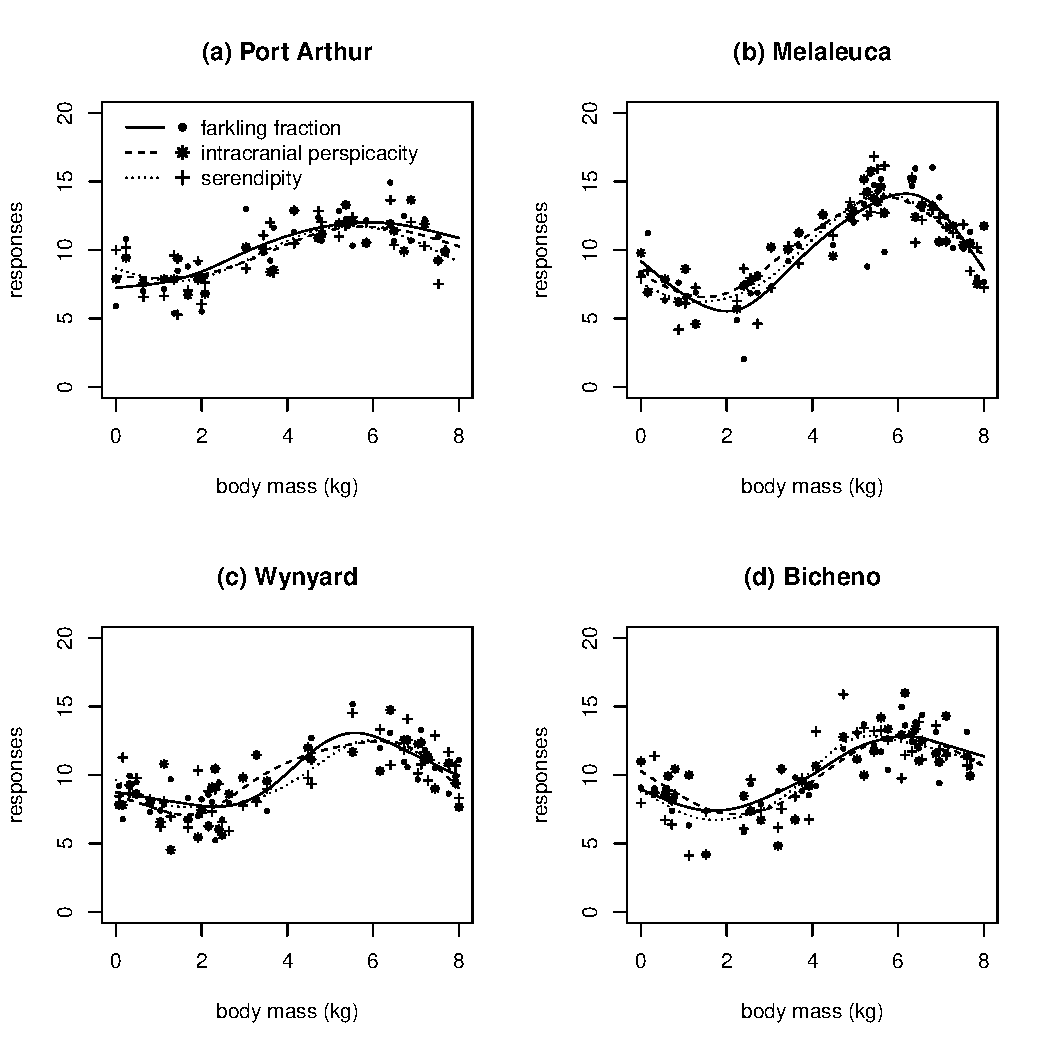
\includegraphics[width=0.95\textwidth]{ltdbFigure}}
\caption{\label{fig:ltdb}
Characteristics of the Lesser Tasmanian Drop Bear (farkling
fraction, intracranial perspicacity and serendipity all in
furlongs per fortnight) plotted against body mass (kilograms).
The observations were made on samples obtained at four locations
in Tasmania. Plotted points represent the raw observed values;
plotted lines represent non-parametric fits to the raw data.}
\end{figure}

% Distinguishing line types and point types.
Another important issue is making sure that line types and
plotting symbols are \emph{distinguishable} in black and white.
Figures appear in the print version of the Journal in black and
white \emph{only}, unless authors specifically request that some or
all of the figures appear in colour and are \emph{willing to pay
a charge} to cover the extra costs that are incurred in printing
colour figures.  So unless you wish to pay this charge --- roughly
speaking \$350 USD per figure --- you should prepare your figures
in black and white, and do this from the very start. (Figures
that are prepared in colour and then converted to black and white
in the printing process usually look awful! Consequently the Journal
does not countenance this practice.)  In particular, lines in
different categories should be distinguished by \emph{line type}
--- solid, dashed, dotted \ldots, and not by colour.  A modest
example is given in Figure~\ref{fig:ltdb}.  Sometimes it is useful,
or perhaps even necessary, to distinguish categories by means of
line \emph{thickness} but proceeding in this way requires a great
deal of care.

Note that colour figures can appear in the online version of the
paper for \emph{free}!  However care must be taken, since \emph{only
one} version of the text of the paper is produced.  Consequently
the online colour figures, and captions and references to figures
in the text, must be structured in such a way as to make sense
both to readers of the black-and-white (print) version and the
colour (online) version.  See \texttt{styleGuide.pdf}, Section
5.1, for a bit more detail.

A common error in respect of tables is making them overly elaborate.
Remember that the purpose of a table is to convey information! If
a table is excessively complex, the reader's eyes will glaze over
and he or she will skip the table, resulting in no information at
all being conveyed.  In particular, if a table is too wide to fit
on a page and has to be rotated 90$^\circ$ in order to be displayed,
then you are trying to put an excessive amount of information into
a single table.  The Journal will henceforth \emph{insist} that
tables fit vertically onto a single page.  If your paper contains
tables that do not satisfy this condition then you will be required
to re-design your table accordingly.  Possibilities for effecting the
re-design include eliminating some of the ``information'', splitting
the table into two or more smaller tables and putting all or part
of the table into the online supplementary material.  An example
of a reasonably perspicuous table is given in Table~\ref{tab:ltdb}.
\begin{table}[htp]
\caption{\label{tab:ltdb}
A load of dingoes' kidneys in respect
of characteristics of the Lesser Tasmanian Drop Bear.  Standard
deviations are given in parentheses after the mean values.}
\centering
\begin{tabular}{|l|r|r|r|r|} \hline
Location & Body mass (kg.) & Farkling & Intracranial & Serendipity \\ 
         &                 & fraction & perspicacity &             \\ \hline
  Port Arthur &  3.95 ( 2.40) & 10.14 ( 2.43) &  9.91 ( 1.99) &  9.81 ( 2.24) \\ 
  Melaleuca   &  4.55 ( 2.41) & 10.48 ( 3.51) & 10.83 ( 2.94) & 10.54 ( 3.30) \\ 
  Wynyard     &  3.87 ( 2.70) &  9.51 ( 2.20) &  9.40 ( 2.44) &  9.50 ( 2.23) \\ 
  Bicheno     &  4.16 ( 2.41) & 10.46 ( 2.44) & 10.44 ( 2.64) & 10.20 ( 2.86) \\ 
   \hline
\end{tabular}
\end{table}
As stated in the ``\textit{ANZJS} Style Guide for Authors''
captions for tables and figures should be left-justified and not
centred unless the text of the caption fits on a single line.
However one-line captions should be centred.  For instance if the
caption of Table~\ref{tab:ltdb} were simply ``Dingoes' kidneys'',
then centring would be preferable.  When the \texttt{anzsauth}
document class is used, captions are automatically centred if
the caption fits on a single line.  (Note that the document
class file \texttt{anzsauth.cls} has recently --- as of
\printdateTeX{2016/11/06} --- been adjusted to make table captions
more similar in appearance to figure captions.  Because of this
adjustment, the centring of one-line table captions is now automatic
whereas, previously, overt measures were required.)

A table or figure that appears in the paper \emph{must} be referred
to in the text, even if only very briefly.  That is, there must
at the very least be something like ``see Figure~17''.  If there
is no such reference, then the corresponding table or figure must
not be included in the paper.

\section{Cross referencing}
\label{sec:crossref}

A facility provided by \LaTeX\ that tends to be underused in
submissions to the Journal is automated cross-referencing as provided
by the \verb!\label{...}! and \verb!\ref{...}! commands.  It is
highly recommended that you learn to make use of these.  They make it
much easier to keep cross-references correct when you revise a paper.
It seems to me to be a good idea to give a label to each section and
subsection, as you are composing it, even if you are not sure you
will be referring to it in other sections.  (There is no \emph{harm}
in inserting a label.)  If you assign labels to sections then you
can easily invite the reader to ``see Section~\ref{sec:figAndTab}''
(as I am about to do below!).  Likewise it is a good idea to give
each figure and table (see Section~\ref{sec:figAndTab}) a label so
as to be able to refer to it via the \verb!\ref{...}!  command.

Only displayed equations that are \emph{actually referred to}
should be numbered (see Section~\ref{sec:eqnNumb}).  If the equation
\emph{is} referred to, then of course you should give it a label so
that you \emph{can} refer to it easily.

My personal practice is to label sections and subsections with labels
of the form \texttt{sec:string}, e.g. ``\verb!\label{sec:intro}!''.
Similarly I form such labels for figures and tables
as \texttt{fig:string} or \texttt{tab:string} (e.g.
\verb!\label{fig:ltdb}! or \verb!\label{tab:ltdb}!) and labels
for equations as \texttt{eq:string} (e.g. \verb!\label{eq:GNZ}!).
I find this practice convenient, but you are of course under no
obligation to follow it.

A practice that I have often seen and that I think should \emph{not}
be indulged in, is to use labels such as ``\texttt{Figure1}''.  There
is \emph{not necessarily} any harm in this, but to a large extent
such a practice defeats the purpose of using \verb!\label{...}! and
\verb!\ref{...}!.  If you decide to change the order in which
figures appear in your paper, then the label ``\texttt{Figure1}''
will probably no longer be appropriate.  At best you will confuse
yourself, and you run a serious risk of getting labels wrong.
Use labels that refer to \emph{content} (in a terse manner, of
course) and let \LaTeX\ handle the assignment of numbers!  If you
insist on using labels like unto ``\texttt{Figure1}'',
then take great care to make sure that the result is correct.

\section{Appendices}
\label{sec:append}

Journal policy is that if there is a single appendix to your document
it should be headed simply `\textbf{Appendix}' (i.e. there should
be no other text in the header and no number).  If the document
has more than one appendix these should be headed \textbf{Appendix
I}, \textbf{Appendix II}, \ldots (i.e. there should be no
other text in the headers, and numbering should be in upper case
Roman numerals).  If you so desire you can place further (centred)
headings underneath the ``\textbf{Appendix}'' headings by using e.g.
\verb!\section*{}!.

Do \emph{not} use the `native' \LaTeX\ command \verb!\appendix!.

To make it easy to supply appendix headers in the appropriate style,
the \texttt{anzsauth} document class provides two new environments:
\texttt{uniqueAppendix} and \texttt{Appendix}.  Use the former
if your document has a single appendix, and the latter if it has
more than one.  The use of the \texttt{Appendix} environment is
illustrated by means of the dummy appendices Appendix~\ref{app:mung},
Appendix~\ref{app:gorp} and Appendix~\ref{app:zephod}.  These mostly
consist of ``Lorem ipsum'' nonsense Latin and are to be found at
the end of this document that you are currently reading.

The \verb!\label{}! and \verb!\ref{}! commands work with appendices
(when there are multiple appendices).  Just put a label within
the relevant \texttt{Appendix} environment and then refer to that
appendix with constructions like ``\verb!See Appendix~\ref{lll}!'',
where ``\verb!lll!'' is the label that you have assigned to the
Appendix in question.  Obviously if you have a unique appendix
you can just say (e.g.) ``See the Appendix \ldots'' and there
is no need for labelling.

In order to illustrate the use of \texttt{uniqueAppendix} I had to
invoke it even though there are actually multiple appendices (four
in all) in this document.  Don't \emph{you} do that!  Do as I say,
not as I do!

The text constituting the illustration of \texttt{uniqueAppendix}
consists of a recapitulation of the foregoing note.

\section{Preparing \LaTeX\ and \BibTeX\ documents}
\label{sec:prepDocs}

\subsection{Editing \LaTeX\ source files}
\label{sec:editors}

There are a number of approaches to preparing your \texttt{*.tex}
and \texttt{*.bib} files. A primary consideration is that you should
use either a general \textbf{text editor}, or a specialised \LaTeX{}
editor for this task.  Do \emph{not} use a word-processing program as
an editor. Using a word-processor introduces a plethora of spurious
non-printing characters which will completely mess things up and
in all likelihood cause the universe to come to an end.

Good text editors include \texttt{vi} or \texttt{vim},
\texttt{emacs}, \texttt{gedit}, \texttt{pico}, \texttt{Crimson},
\texttt{Notepad++},~\ldots\ .  Good editors will have support
for editing of \LaTeX{} such as syntax highlighting and code
completion. The Windows\texttrademark\ editors \texttt{Notepad}
and \texttt{Wordpad} are distinctly inferior in this respect.

Among a number of possible specialised \LaTeX{} editors, one that
has been highly recommended to me by several reliable sources
is \texttt{TeXstudio}. This is an open-source, multi-platform,
fully-featured editor for \LaTeX{}. It allows for easy processing of
documents, has support for inclusion of a vast range of characters,
provides auto-completion of \LaTeX{} commands, has a built-in pdf
viewer and a number of other helpful facilities. Other similar
programs are \texttt{Texmaker} and (Windows\texttrademark\ only)
\texttt{WinEdt}.

Users of Windows\texttrademark\ will almost surely make use of
\LaTeX\ via \MiKTeX.  This is free open source software, and is
readily available and easy to install.

The integrated development environment (IDE) \texttt{proTeXt} is
described as being ``an easy-to-install \TeX{} distribution for
Windows\texttrademark, based on \texttt{MiKTeX}'', ``which adds
the \texttt{TeXstudio} front end to MiKTeX''.  Some authors may
find it helpful.

\subsection{Processing source files}
\label{sec:procBib}

One advantage of using specialised \LaTeX{} editors is the ease of
processing (``compiling'') source files, particularly in respect of
handling \BibTeX{} files. Such processing can be accomplished with
a single mouse click when \texttt{TeXstudio}, for example, is used.

If you use a ``general'' text editor and process the source
of your document by means of command line instructions, the procedure
requires more steps.  To compile a document which uses the \BibTeX\
protocols described in Section~\ref{sec:useBib}, you need to run
\LaTeX\ on the document, then run \BibTeX, then run \LaTeX\ again
(possibly several times) until it stops complaining that labels
may have changed.  Something like:
\begin{verbatim}
    latex magnumOpus
    bibtex magnumOpus
    latex magnumOpus
    latex magnumOpus
       .
       .
       .
\end{verbatim}
(In the foregoing ``\texttt{magnumOpus}'' represents the \emph{stem}
of the name of the file ``\texttt{magnumOpus.tex}'' containing
the source of your paper.  You may wish to use \texttt{pdflatex}
rather than \texttt{latex} as your ``compilation'' command.)

Whether you are using a general or a specialised editor, if you get
errors or warnings from the \texttt{bibtex} command you must edit
the \texttt{*.bib} file and fix whatever was causing the errors
(things like commas being left out).  After fixing the problem,
process the file again (if you are using a specialised editor)
or run \texttt{bibtex} again (otherwise).  After the initial
learning period, the processing procedure all goes very smoothly.
Try it. It really does make life a lot easier and saves a lot of
time and errors. Once you get used to it you'll never look back.

\section{What to do with \texttt{anzsauth.cls} and \texttt{anzsj.bst}?}
\label{sec:wheretoshove}

I have been told that some authors don't know what to do with the
files (to be found in \texttt{anzsauth.zip}) referred to in the
title of this section.  In some sense, it's really very simple:  all
you need to do is to place these files in a directory (``folder''
if you want to \emph{be} that way!) where \LaTeX\ can find them.
A very simple way to accomplish this is to place these files in
the ``working directory'' that contains the source \texttt{*.tex}
file for your paper.  This is a bit untidy, but.

Doing things in a tidy organised way is a bit harder and is very
much dependent on your operating system and your \TeX\ installation.
The plethora of possibilities involved is what makes things ``a
bit harder''.  (Puts me in mind of a line from a Joni Mitchell song:
``\ldots the kind of crazy you get from having too much choice''.)
Because of this plethora of possibilities I cannot say very much
here.  You are advised to seek local guidance.  Google\texttrademark\
provides some information, but the instructions that you find
are often a bit confusing and sometimes a bit contradictory.
Getting ``local advice'' is best, if this is possible.

On Linux systems you can place the files in appropriate
sub-directories of the appropriate ``\texttt{texmf}'' directory.
You may need to search around a bit to find where this latter
directory lives.  If your \TeX\ installation is \texttt{texlive},
the relevant directory is actually called \texttt{texmf-dist}.
Google\texttrademark\ may help you track things down.

Another procedure is to put these files in a directory (or in
directories) that you create under your home directory, and make
use of the \emph{environment} variables \texttt{TEXINPUTS} and
\texttt{BSTINPUTS} to tell \LaTeX\ where to find them.  This is
what I do personally.  I won't try to go into the details.  It
is possible that Google\texttrademark\ will help.

On Mac OSX\texttrademark\ systems you should (apparently)
put \texttt{anzsauth.cls} in a directory
\begin{verbatim}
    ~/Library/texmf/tex/latex/anzsauth
\end{verbatim}
and put \texttt{anzsj.bst} in
\begin{verbatim}
    ~/Library/texmf/bibtex/bst/anzsj
\end{verbatim}
where ``\verb!~!'' means your home directory.  (Of course!)
Take the foregoing advice with a grain of salt --- I don't use
Mac OSX\texttrademark\ and I have not tested the advice that
I have given.

As regards Windows\texttrademark\ systems, I can't help you at
all.  I don't \emph{do} Windows\texttrademark!

\section{Concluding comments}
\label{sec:concComm}

This document contains guidance on how to prepare a paper for
submission to \textit{ANZJS} by making use of the \texttt{anzsauth}
document class for \LaTeX.  You will find that by making use of this
document class and following the advice that is provided in the
foregoing material, you will be able to produce a paper that meets
the Journal's requirements and that requires much less revision and
adjustment than it otherwise might, thus speeding up the publication
process considerably.

This document also emphasises the importance of good exposition and
correct use of the English language.  The Journal has very high,
and strictly enforced, standards in this regard.  Please pay close
attention to this requirement and give careful thought to the way
in which you express yourself.  Doing so will, again, speed up the
publication process for you.

The accompanying file \texttt{protoType.tex} forms a template for
\LaTeX\ source files for papers that are to be submitted to the
Journal.  When preparing your own \LaTeX\ source file, you should
imitate the structure of the template closely.  You may find that an
effective way to proceed is to edit the template, \textit{mutatis
mutandis}, replacing authors' names, the title of the paper,
the abstract (summary) and the actual content as is appropriate.
\emph{Please} remove extraneous bits and pieces from the prototype
file when converting it into your own paper.  Don't leave material
that is relevant only to the prototype (e.g. comments advising
you how to format your paper) lying around.  Tidy up!  This makes
processing your paper for publication much easier (and quicker!).
In respect of tidyness I draw your attention to the last paragraph
of this section (keep the typescript in your source file tidy!).

With regard to removing extraneous material, it turns out to be
expedient for me to mention that the disclaimer at the end of the
footnotes on the title page of this document should \emph{not} be
included when you adapt the prototype source file to your own uses.
That disclaimer applies to \emph{this paper}, i.e. ``\textbf{How I
rose from the dead in my spare time and so can you}''.  The Journal
does \emph{not} require you to include such a disclaimer in
\emph{your} paper, nor should you do so.

Although it is not necessary to prepare the initial submission using
the \texttt{anzsauth} document class, it is very important that
the final version that you submit (after provisional acceptance of
your paper) should conform to the Journal's requirements.  This is
much more likely to be the case if you use the \texttt{anzsauth}
document class.  It is likely to be less work for you if you make
use of this document class and of the template from the outset,
if this is at all possible. Note that it \emph{is} necessary for
the initial submission to be double spaced and to be line-numbered.
These requirements are greatly facilitated by using the required
document class.  See page \pageref{pg:dsln}.

It is often the case that the Technical Editor will wish to make
some minor (or sometimes major!) adjustments to the \LaTeX\ source
file that you provide, before putting the paper into production.
This saves having to send the paper back to authors, yet one more
time, to get these adjustments made.  The process of making these
adjustments is a \emph{whole lot} easier if the source file is
constructed in a tidy and comprehensible manner.  Use appropriate
line breaks (keeping lines to a length of, e.g., at most 80
characters) and ensure that there is appropriate \emph{spacing}
between mathematical constructions.  Do not embed \LaTeX\ commands
to produce displayed equations in on-running lines of text.  All of
this will have of course absolutely no impact on the \emph{output}
file produced by compiling the \LaTeX\ source, but it simplifies
the process of modifying and adjusting this source by orders of
magnitude.

\begin{Appendix}
\label{app:mung}

This is an appendix. \lipsum[1]

\end{Appendix}

\begin{Appendix}
\label{app:gorp}

This is another appendix. \lipsum[2]

\end{Appendix}

\begin{Appendix}
\label{app:zephod}
\begin{center}
Zephod Beeblebrox
\end{center}

\emph{This} appendix was written by Zephod Beeblebrox, but he didn't
actually have anything to say. \lipsum[3]
\end{Appendix}

% Note that this usage of the uniqueAppendix environment is wrong
% here, since there are actually multiple appendices.  But, hey,
% what can you do?  (If you want to illustrate the use of both
% environments in a single document.)
\begin{uniqueAppendix}
This is what you should get if you had only \emph{one} appendix.
Since this document has several appendices (four, actually) the
use of the \texttt{uniqueAppendix} environment is completely
inappropriate here.  It is included for illustrative purposes
only.  I needed to illustrate syntax to be used both for multiple
and unique appendices, but obviously one cannot have a single
document in which there is a unique appendix and in which there are
multiple appendices!  (That would violate the, uh, law of small
numbers. \verb! :-) !)  Consequently I was forced to include an
inappropriate example of the use of \texttt{uniqueAppendix}.

I reiterate:  Use the \texttt{uniqueAppendix} environment if there is
only one appendix to your document.  Use the \texttt{Appendix}
environment if there are two or more appendices to your document.
\end{uniqueAppendix}

%\nocite{PussyRiot2014}
%\nocite{Nixon1984}
%\nocite{Turner2017}
%\nocite{Brillinger2007}

\newpage
\bibliographystyle{anzsj}
\bibliography{protoRefs}
\end{document}
